% LaTeX source for ``Think Stats:
% Probability and Statistics for Programmers''
% Copyright 2010  Allen B. Downey.

% License: Creative Commons Attribution-Share Alike 3.0 Unported
% http://creativecommons.org/licenses/by-sa/3.0/
%

%\documentclass[10pt,b5paper]{book}
\documentclass[10pt]{book}
\usepackage[width=5.5in,height=8.5in,
  hmarginratio=3:2,vmarginratio=1:1]{geometry}

% for some of these packages, you might have to install
% texlive-latex-extra (in Ubuntu)

\usepackage{pslatex}
\usepackage{url}
\usepackage{fancyhdr}
\usepackage{graphicx}
\usepackage{amsmath, amsthm, amssymb}
\usepackage{exercise}                        % texlive-latex-extra
\usepackage{makeidx}
\usepackage{setspace}
\usepackage{hevea}                           
\usepackage{upquote}

\title{Think Stats}
\newcommand{\thetitle}{Think Stats: Probability and Statistics for Programmers}
\newcommand{\theversion}{1.0.0}

% these styles get translated in CSS for the HTML version
\newstyle{a:link}{color:black;}
\newstyle{p+p}{margin-top:1em;margin-bottom:1em}
\newstyle{img}{border:0px}

% change the arrows in the HTML version
\setlinkstext
  {\imgsrc[ALT="Previous"]{back.png}}
  {\imgsrc[ALT="Up"]{up.png}}
  {\imgsrc[ALT="Next"]{next.png}} 

\makeindex

\begin{document}

\frontmatter

% LATEXONLY

\input{latexonly}

\newtheorem{ex}{Exercise}[chapter]

\begin{latexonly}

\renewcommand{\blankpage}{\thispagestyle{empty} \quad \newpage}

%\blankpage
%\blankpage

% TITLE PAGES FOR LATEX VERSION

%-half title--------------------------------------------------
\thispagestyle{empty}

\begin{flushright}
\vspace*{2.0in}

\begin{spacing}{3}
{\huge Think Stats: Probability and Statistics for Programmers}\\
{\Large }
\end{spacing}

\vspace{0.25in}

Version \theversion

\vfill

\end{flushright}

%--verso------------------------------------------------------

\blankpage
\blankpage
%\clearemptydoublepage
%\pagebreak
%\thispagestyle{empty}
%\vspace*{6in}

%--title page--------------------------------------------------
\pagebreak
\thispagestyle{empty}

\begin{flushright}
\vspace*{2.0in}

\begin{spacing}{3}
{\huge Think Stats}\\
{\Large Probability and Statistics for Programmers}
\end{spacing}

\vspace{0.25in}

Version \theversion

\vspace{1in}


{\Large
Allen Downey\\
}


\vspace{0.5in}

{\Large Green Tea Press}

{\small Needham, Massachusetts}

%\includegraphics[width=1in]{figs/logo1.eps}
\vfill

\end{flushright}


%--copyright--------------------------------------------------
\pagebreak
\thispagestyle{empty}

{\small
Copyright \copyright ~2010 Allen Downey.


\vspace{0.2in}

\begin{flushleft}
Green Tea Press       \\
9 Washburn Ave \\
Needham MA 02492
\end{flushleft}

Permission is granted to copy, distribute, and/or modify this document
under the terms of the Creative Commons Attribution-Share Alike 3.0 Unported
License, which is available at \url{creativecommons.org/licenses/by-sa/3.0/}.

The original form of this book is \LaTeX\ source code.  Compiling this
code has the effect of generating a device-independent representation
of a textbook, which can be converted to other formats and printed.

The \LaTeX\ source for this book is available from
\url{www.thinkstatsbook.com}.

The cover for this book is based on a photo by Paul Friel
(\url{flickr.com/people/frielp/}), who made it available under
the Creative Commons Attribution license.  The original photo
is at \url{flickr.com/photos/frielp/11999738/}.

\vspace{0.2in}

} % end small

\end{latexonly}


% HTMLONLY

\begin{htmlonly}

% TITLE PAGE FOR HTML VERSION

{\Large \thetitle}

{\large Allen B. Downey}

Version \theversion

\setcounter{chapter}{-1}

\end{htmlonly}


\chapter{Preface}

\section*{Programming is a pedagogic wedge}



Allen B. Downey \\
Needham MA\\

Allen Downey is an Associate Professor of Computer Science at 
the Franklin W. Olin College of Engineering.




%\section*{Acknowledgements}



\section*{Contributor List}

\index{contributors}

If you have a suggestion or correction, please send email to 
{\tt downey@allendowney.com}.  If I make a change based on your
feedback, I will add you to the contributor list
(unless you ask to be omitted).

If you include at least part of the sentence the
error appears in, that makes it easy for me to search.  Page and
section numbers are fine, too, but not quite as easy to work with.
Thanks!

\small

\begin{itemize}

\item 

% ENDCONTRIB

\end{itemize}

\normalsize

\clearemptydoublepage

% TABLE OF CONTENTS
\begin{latexonly}

\tableofcontents

\clearemptydoublepage

\end{latexonly}

% START THE BOOK
\mainmatter


\chapter{Statistical thinking for programmers}

This book is about turning data into knowledge.  Data is cheap (at
least relatively); knowledge is harder to come by.

I will present three related pieces:

\begin{description}

\item[Probability] is the study of random events.  Most people have an
  intuitive understanding of degrees of probability, which is why we
  can use words like ``probably'' and ``unlikely'' without special
  training, but we will talk about how to make quantitative claims
  about those degrees.

\item[Statistics] is the discipline of using data samples to support
  claims about populations.  Most statistical analysis is based on
  probability, which is why these pieces are usually presented
  together.

\item[Computation] is a tool that is well-suited to quantitative
  analysis, and computers are commonly used to process statistics.
  Also (and more importantly for this book) computational experiments
  are useful for exploring concepts in probability and statistics.

\end{description}

The thesis of this book is that if you know how to program, you can
use that skill to help you understand probability and statistics.
These topics are often presented from a mathematical perspective, and
that approach works well for some people.  But some important ideas
in this area are hard to work with mathematically and relatively
easy to approach computationally.

Both approaches have merits, and the ideal might combine both, but
the goal of this book is to explore the computational path.

The rest of this chapter presents a case study motivated by a question
I heard when my wife and I were expecting our first child: do first
babies tend to arrive late?

\section{Do first babies arrive late?}

If you Google this question, you will find plenty of discussion.
Some people claim it's true, others say it's a myth, and some people
say it's the other way around: first babies come early.

In many of these discussions, people provide data to support their
claims.  I found many examples like these:

\begin{quote}

``My two friends that have given birth recently to their first babies,
BOTH went almost 2 weeks overdue before going into labour or being
induced.''

``My first one came 2 weeks late and now I think the second one is
going to come out two weeks early!!''

``I don't think that can be true because my sister was my mother's
first and she was early, as with many of my cousins.''

\end{quote}

Reports like these are called {\bf anecdotal evidence} because they
are based on data that is unpublished and usually personal.  In casual
conversation, there is nothing wrong with anecdotes, so I don't mean
to pick on the people I quoted.

But we might want evidence that is more persuasive and
an answer that is more reliable.  By those standards, anecdotal
evidence usually fails, because:

\begin{description}

\item[Small number of observations:] If the gestation period is longer
  for first babies, the difference is probably small compared to the
  natural variation.  In that case, we might have to compare a large
  number of pregnancies to be sure there is really a difference (or
  not).

\item[Selection bias:] People who join a discussion of this question
  might be interested because their first babies were late.  In that
  case the process of selecting data would bias the results.

\item[Confirmation bias:] People who believe the claim might be more
  likely to contribute examples that confirm it.  People who doubt the
  claim are more likely to cite counterexamples.

\item[Inaccuracy:] Anecotes are often personal stories that are
  (deliberately or not) misremembered, misrepresented, repeated
  inaccurately, etc.

\end{description}

So how can we do better?

\section{A statistical approach}

To address the limitations of anecdotes, we will use the tools
of statistics, which include:

\begin{description}

\item[Data collection:] We will use data from a large national survey
  that was designed explicitly with the goal of generating
  statistically valid inferences about the U.S. population.

\item[Descriptive statistics:] We will generate statistics that
  summarize the data concisely, and evaluate different ways to
  visualize data.

\item[Exploratory data analysis:] We will examine the data looking for
  patterns, differences, and other features that address the questions
  we are interested in.  At the same time we will check for
  inconsistencies and identify limitations.

\item[Hypothesis testing:] Where we see apparent effects (like a
  difference between two groups), we will evaluate whether the effect
  is likely to be real, or whether it might have happened by chance.

\item[Estimation:] We will use measurements in the dataset to estimate
  characteristics of the general population.

\end{description}

By performing these steps with care to avoid common pitfalls, we can
reach conclusions that are more justifiable and more likely to be
correct.


\section{The National Survey of Family Growth}

Since 1973 the U.S. Centers for Disease Control and Prevention (CDC)
have conducted the National Survey of Family Growth (NSFG),
which is intended to gather ``information on family life, marriage and
divorce, pregnancy, infertility, use of contraception, and men's and
women's health. The survey results are used ... to plan health services and
health education programs, and to do statistical studies of families,
fertility, and health.''\footnote{See
  \url{cdc.gov/nchs/nsfg.htm}.}

We will use data collected by this survey to investigate whether first
babies tend to come late, and other questions.  In order to use this
data effectively, we have to understand the design of the study.

The NSFG is a {\bf cross-sectional} study, which means that it
captures a snapshot of a group at a point in time.  The most
common alternative is a {\bf longitudinal} study, which observes a
group repeatedly over a period of time.

The NSFG has been conducted seven times; each deployment is called
a {\bf cycle}.  We will be using data from Cycle 6, which was
conducted from January 2002 to March 2003.

The goal of the survey is to draw conclusions about a
{\bf population}; the target population of the NSFG is people in
the United States aged 15-44.

The people who participate in a survey are called {\bf respondents}.
In general, cross-sectional studies are meant to be {\bf
  representative}, which means that every member of the target
population has an equal chance of participating.  Of course that ideal
is hard to achieve in practice, but people who conduct surveys come as
close as they can.

The NSFG not representative; instead it is deliberately {\bf
  oversampled}.  The designers of the study recruited three
groups---Hispanics, African-Americans and teenagers---at rates higher
than their representation in the U.S. population.
The reason for oversampling is to make sure that the number of
respondents in each of these groups is large enough to draw valid
statistical inferences.

Of course, the drawback of oversampling is that it is not as easy
to draw conclusions about the general population based on statistics
from the survey.  We will come back to this point later.

\begin{ex}

Although the NSFG has been conducted seven times, it is not a
longitudinal study.  Read the Wikipedia pages
\url{wikipedia.org/wiki/Cross-sectional_study}
and
\url{wikipedia.org/wiki/Longitudinal_study}
to make sure you understand why not.

\end{ex}

\begin{ex}

In this exercise, you will download data from the NSFG and do some
exploratory data analysis.

\begin{enumerate}

\item Go to \url{thinkstatsbook.com/nsfg.html}.  Read the terms of
use for this data and click ``I accept these terms'' (assuming that you do).

\item Download the files named {\tt 2002FemResp.dat.gz} and {\tt
  2002FemPreg.dat.gz}.  The first is the respondent file, which contains
  one line for each of the 7,643 female respondents.
  The second file contains one line for each pregnancy reported by a
  respondent.

\item Online documentation of the survey is at
  \url{nsfg.icpsr.umich.edu/cocoon/WebDocs/NSFG/public/index.htm}.
  Browse the sections in the left navigation bar to get a sense of
  what data are included.  You can also read the questionnaires
  at \url{cdc.gov/nchs/data/nsfg/nsfg_2002_questionnaires.htm}.

\item The web page for this book provides code to process the data
  files from the NSFG.  Download \url{thinkstatsbook.com/survey.py}
  and run it in the same directory you put the data files in.  It
  should read the data files and print the number of lines in each:

\begin{verbatim}
Number of respondents 7643
Number of pregnancies 13593
\end{verbatim}

\item Browse the code to get a sense of what it does.  The next
section explains how it works.

\end{enumerate}

\end{ex}

\section{Tables and records}

The poet-philosopher Steve Martin once said:

\begin{quote}
``Oeuf'' means egg, ``chapeau'' means hat.  It's like those French
  have a different word for everything.
\end{quote}

Like the French, database programmers speak a slightly
different language, and since we're working with a database we need
to learn some vocabulary.

Each line in the respondents file contains information about one
respondent.  This information is called a {\bf record}.  The
variables that make up a record are called {\bf fields}.  A
collection of records is called a {\bf table}.

If you read {\tt survey.py} you will see class definitions for {\tt
  Record}, which is an object that represents a record, and {\tt
  Table}, which represents a table.

There are two subclasses of
{\tt Record}, {\tt Respondent} and {\tt Pregnancy}, which will
contain records from the respondent and pregnancy tables.
For the time being, these classes are empty; in particular, there
is no {\tt init} method to initialize their attributes.  Instead
we will use {\tt Table.MakeRecord} to convert a line of text into
a {\tt Record} object.

There are also two subclasses of {\tt Table}, {\tt Respondents}
and {\tt Pregnancies}.  The {\tt init} method in each class
specifies the default name of the data file and the type of
record to create.  Each {\tt Table} object has an attribute
named {\tt records}, which is a list of {\tt Record} objects.

For each {\tt Table}, the {\tt GetFields} method returns
a list of tuples that specify the fields from the record that
will be stored as attributes in each {\tt Record} object.

For example, here is {\tt Pregnancies.GetFields}:

\begin{verbatim}
    def GetFields(self):
        return [
            ('caseid', 1, 12, int),
            ('prglength', 275, 276, int),
            ('outcome', 277, 277, int),
            ('birthord', 278, 279, int),
            ('finalwgt', 423, 440, float),
            ]
\end{verbatim}

The elements of these tuples are:

\begin{description}

\item[field:] The name of the attribute where the field
will be stored.  Most of the time I use the names from the
NSFG codebook, converted to all lower case.

\item[start:] The index of the starting location for this
field.  You can look up these indices in the NSFG codebook
at \url{nsfg.icpsr.umich.edu/cocoon/WebDocs/NSFG/public/index.htm}.
For example, the indices for {\tt caseid} are
1--12.

\item[end:] The index of the ending location for this
field.

\item[conversion function:] A function that takes a string
and converts it to an appropriate type.  You can use built-in
functions like {\tt int} and {\tt float} or a user-defined
function.  If the conversion fails, the attribute gets the
string value {\tt 'NA'}.  If you don't want to convert a
field, you can provide an identity function or use {\tt str}.

\end{description}

For pregnancy records, we extract the following variables:

\begin{description}

\item[caseid] is the integer ID of the associated respondent.

\item[prglength] is the integer duration of the pregnancy in weeks.

\item[outcome] is an integer code for the outcome of the pregnancy.
The code 1 indicates a live birth.

\item[birthord] is the integer birth order of each live birth;
for example, the code for a first child is 1. 
For outcomes other than live birth, this field is blank.

\item[finalwgt] is the statistical weight associated with the respondent.
It is a floating-point value that indicates the number of people in
the U.S. population this respondent represents.  Members of undersampled
groups have higher weights.

\end{description}

If you read the casebook carefully, you will see that most of these
variables are {\bf recodes}, which means that they are not part
of the {\bf raw data} collected by the survey, but they are
calculated using the raw data.

For example, {\tt prglength} for live births is equal to the raw
variable {\tt wksgest} (weeks of gestation) if it is available;
otherwise it is estimated using {\tt mosgest * 4.33} (months of
gestation times the average number of weeks in a month).

Recodes are often based on logic that checks the consistency and
accuracy of the data.  In general it is a good idea to use recodes
unless there is a compelling reason to process the raw data
yourself.

\begin{ex}

In this exercise you will write a program to explore the data
in the Pregnancies table.

\begin{enumerate}

\item In the directory where you put {\tt survey.py} and the
data files, create a file named \verb"first.py" and
type or paste in the following code:

\begin{verbatim}
import survey
table = survey.Pregnancies()
table.ReadRecords()
print 'Number of pregnancies', len(table.records)
\end{verbatim}

The result should be 13593 pregnancies.

\item Write a loop that iterates \verb"table" and counts
the number of live births.  Find the documentation of {\tt outcome}
and confirm that your result is consistent with the summary
in the documentation.

\item Modify the loop to partition the live birth records into
two groups, one for first babies and one for the others.  Again,
read the documentation of {\tt birthord} to see if your results
are consistent.

When you are working with a new dataset, these kinds of checks
are useful for finding errors and inconsistencies in the data,
detecting bugs in your program, and checking your understanding
of the way the data are encoded.

\item Compute the average pregnancy length (in weeks) for first
babies and others.  Is there a difference between the groups?  How
big is it?

Note: For now we are ignoring the {\tt finalwgt} variable.

\end{enumerate}

You can download a solution to this exercise from
\url{thinkstatsbook.com/first.py}.

\end{ex}

\section{Significance}

In the previous exercise, you compared the gestation
period for first babies and others, and if things worked out,
you found that first babies are born about 13 hours later,
on average.

A difference like that is called an {\bf apparent effect};
that is, there might be something going on, but we are not
yet sure.  There are several questions we still want to ask:

\begin{itemize}

\item If the two groups have different means, what about other {\bf
  summary statistics}, like median and variance?  Can we be more
  precise about how the groups differ?

\item Is it possible that the difference we saw could occur by chance,
  even if the groups we compared were actually the same?  If so,
  we would conclude that the effect was not {\bf statistically
    significant}.

\item Is it possible that the apparent effect is due to sample bias or
  some other error in the experimental setup?  If so, then we might
  conclude that the effect is an {\bf artefact}; that is, something we
  created (by accident) rather than found. 

\end{itemize}

We will address these questions in the next few chapters.

\section{Glossary}

\begin{description}

\item[anecdotal evidence:] Evidence, often personal, that is collected
  casually rather by a well-designed study.

\item[population:] A group we are interested in studying, often a
  group of people, but the term is also used for animals, vegetables
  and minerals\footnote{If you don't recognize this phrase, see
    \url{wikipedia.org/wiki/Twenty_Questions}.}.

\item[cross-sectional study:] A study that collects data about a
population at a particular point in time.

\item[longitudinal study:] A study that follows a population over
time, collecting data from the same group repeatedly.

\item[respondent:] A person who responds to a survey.

\item[sample:] The subset of a population used to collect data.

\item[representative:] A sample is representative if every member
of the population has the same chance of being in the sample.

\item[oversampling:] The technique of increasing the representation
of a sub-population in order to avoid errors due to small sample
sizes.

\item[record:] In a database, a collection of information about
a single person or other object of study.

\item[field:] In a database, one of the named variables that makes
up a record.

\item[table:] In a database, a collection of records.

\item[raw data:] Values collected and recorded with little or no
checking, calculation or interpretation.

\item[recode:] A value that is generated by calculation and other
logic applied to raw data.

\item[summary statistic:] The result of a computation that reduces
a dataset to a single number (or at least a smaller set of numbers)
that captures some characteristic of the data.

\item[apparent effect:] A measurement or summary statistic that
suggests that something interesting is happening.

\item[statistically significant:] An apparent effect is statistically
  significant if it is unlikely to occur by chance.

\item[artefact:] An apparent effect that is caused by bias,
  measurement error, or some other kind of error.

\end{description}

\section{Exercises}

\begin{ex}

The best way to learn about statistics is to work on a project you are
interested in.  Is there a question like, ``Do first babies arrive
late,'' that you would like to investigate?

Think about questions you find personally interesting, or items of
conventional wisdom, or controversial topics, or questions that have
political consequences, and see if you can formulate a question that
lends itself to statistical inquiry.

Now start looking for data to help you address the
question.  Governments are good sources because data from
public research is often freely available\footnote{On the day
I wrote this paragraph, a court in the UK ruled that the
Freedom of Information Act applies to scientific research data.}.

Another way to find data is Wolfram Alpha, which is a curated
collection of good-quality datasets at \url{wolframalpha.com}.
Results from Wolfram Alpha are subject to copyright
restrictions; you might want to check the terms before you commit
yourself.

Google and other search engines can also help you find data, but it
can be harder to evaluate the quality of resources on the web.

If it seems like someone has answered your question, look closely to
see whether the answer is justified.  There might be flaws in the data
or the analysis that make the conclusion unreliable.  In that case you
could perform a different analysis of the same data, or look for a
better source of data.

If you find a published paper that addresses your question, you
should be able to get the raw data.  Many authors make their data
available on the web, but for sensitive data you might have to
write to the authors, provide information about how you plan to use
the data, or agree to certain terms of use.  Be persistent!

\end{ex}


\chapter{Descriptive statistics}

\section{Means and averages}
\label{mean}

In the previous chapter, I mentioned three summary statistics---mean,
variance and median---without explaining what they are.  So before
we go any farther, let's take care of that.

If you have a sample of $n$ values, $x_i$, the mean, $\mu$, is
the sum of the values divided by the number of values; in other words

\[ \mu = \frac{1}{n} \sum_i x_i \]

\begin{ex}
For the exercises in this chapter, create two file:

\begin{description}

\item[{\tt thinkstats.py}]: This file will contain general-purpose
functions we will use throughout the book.

\item[{\tt descriptive.py}]: This file will contain code specific
to the exercises in this chapter.

\end{description}

In {\tt thinkstats.py} write a Python function named {\tt Mean} that
takes a sequence of numbers and returns their mean.  Hint: the result
should be a floating-point value even if the numbers are integers.

In {\tt descriptive.py} write code that tests {\tt Mean}.
\end{ex}

The words ``mean'' and ``average'' are sometimes used interchangeably,
but I will maintain this distinction:

\begin{itemize}

\item The ``mean'' of a sample is the summary statistic computed with
  the previous formula.

\item An ``average'' is one of many summary statistics you might
  choose to describe the typical value, or the expected value, or the
  {\bf central tendency} of a sample.  

\end{itemize}

Sometimes the mean is a good description of a set of values.  For
example, apples are all pretty much the same size (at least the ones
sold in supermarkets).  So if I buy 6 apples and the total weight is 3
pounds, it would be a reasonable summary to say they are about a half
pound each.

But pumpkins are more diverse.  Suppose I grow several varieties in my
garden, and one day I harvest three decorative pumpkins that are 1
pound each, two pie pumpkins that are 3 pounds each, and one Atlantic
Giant\textregistered~pumpkin that weighs 591 pounds.  The mean of
this sample is 100 pounds, but if I told you ``The average pumpkin
in my garden is 100 pounds,'' that would be wrong, or at least
misleading.

In this example, there is no meaningful average because
there is no typical pumpkin.

\section{Variance}

If there is no single number that summarizes pumpkin weights,
we can do a little better with two numbers: mean and {\bf variance}.

In the same way that the mean is intended to describe the central
tendency, variance is intended to describe the ``spread''.
The variance of a set of values is

\[ \sigma^2 = \frac{1}{n} \sum_i (x_i - \mu)^2 \]

The term $x_i - \mu$ is called the ``deviation from the mean,'' so
variance is the mean squared deviation, which is why it is denoted
$\sigma^2$.  The square root of variance, $\sigma$, is called the {\bf
  standard deviation}.

\begin{ex}
In {\tt thinkstats.py} write a function named {\tt Var} that takes a
sequence of numbers and returns their variance.

In {\tt descriptive.py} write code that
computes the variance of the pumpkin data.
\end{ex}

\begin{ex}
Reusing code from {\tt survey.py} and {\tt first.py}, compute the
variance of gestation time for first babies and others.  Does it look
like the spread is the same for the two groups?
\end{ex}

\begin{ex}
Compute the standard deviation of the pooled data (first babies
and others).  How big is the difference between the
means compared to the standard deviation?  What does this comparison
suggest about the statistical significance of the difference?
\end{ex}

If you have prior experience, you might have seen a 
formula for variance with $n-1$ in the denominator, rather than $n$.
This statistic is called the ``sample variance,'' and it is used
to estimate the variance in a population using a sample.  We will
come back to this when we talk about estimation.

\section{Distributions}

Summary statistics are concise, but dangerous, because they obscure
the data.  An alternative is to look at the {\bf distribution} of the
data, which describes how often each value appears.

The most common representation of a distribution is a {\bf histogram},
which is a graph that shows the frequency or probability
of each value.  

In this context, {\bf frequency} means the number of times a value
appears in a dataset---it has nothing to do with the pitch of a sound
or tuning of a radio signal.  A {\bf probability} is a frequency expressed
as a fraction of the sample size, $n$.

In Python, an efficient way to compute frequencies is with a dictionary.
Given a sequence of values, $t$:

\begin{verbatim}
hist = {}
for x in t:
    hist[x] = hist.get(x, 0) + 1
\end{verbatim}

So {\tt hist} is a dictionary that maps from values to frequencies.
To get from frequencies to probabilities, we divide through by $n$,
which is called {\bf normalization}:

\begin{verbatim}
n = float(len(t))
pmf = {}
for x, freq in hist.items():
    pmf[x] = hist[x] / n
\end{verbatim}

The normalized histogram is called a {\bf pmf}, which stands for
``probability mass function;''  that is, it's a function that
maps from values to probabilities (I'll explain ``mass'' later).

It might be confusing to call a Python dictionary a function.  In
mathematics, a function is a mapping from one set of values to
another.  In Python, we {\em usually} represent mathematical functions
with function objects, but in this case we are using a dictionary
(which is also called a ``map,'' if that helps).

\begin{ex}
Create a file named {\tt Pmf.py} and write a definition for a class
named {\tt Hist} that represents a histogram with a dictionary
that maps from values to frequencies.

Write a function named {\tt MakeHist} that takes a sequence of
values and returns a Hist object.

Write a method named {\tt Freq} that takes a value and returns
the corresponding frequency, or 0
if the value hasn't appeared.  Write tests for your code.
\end{ex}


\begin{ex}
In {\tt Pmf.py}, write a definition for a class named {\tt Pmf} that
represents a probability mass function with a dictionary that maps
from values to probabilities.

Write a function called {\tt MakePmf} that takes a sequence of
values and returns their pmf.

Write a method called {\tt Prob} that
takes a value and returns the corresponding probability, or 0
if the value has frequency 0.  Write tests to test your code.
\end{ex}


\section{Plotting histograms}

There are a number of Python packages for making figures and graphs.
The one I will use in the book is {\tt pyplot}, which is part of
the {\tt matplotlib} package at \url{matplotlib.sourceforge.net}.

This package is included in many Python installations.  To see whether
you have it, launch the Python interpreter and run:

\begin{verbatim}
import matplotlib.pyplot as plt
plt.pie([1,2,3])
plt.show()
\end{verbatim}

If you have {\tt matplotlib} you should see a simple pie chart;
otherwise you will have to install it.

The {\tt import...as} statement lets you import a package and give
it a nickname, which is convenient if the name of the package is long.
I will use the nickname {\tt plt} to be consistent with the examples
in the {\tt pyplot} documentation.

Histograms and pmfs are most often plotted as bar charts.  The
{\tt pyplot} function to draw a bar chart is {\tt bar}.

Figure~\ref{nsfg_hist} shows histograms of the pregnancy lengths for
first babies and others.

\begin{figure}
% descriptive.py
\centerline{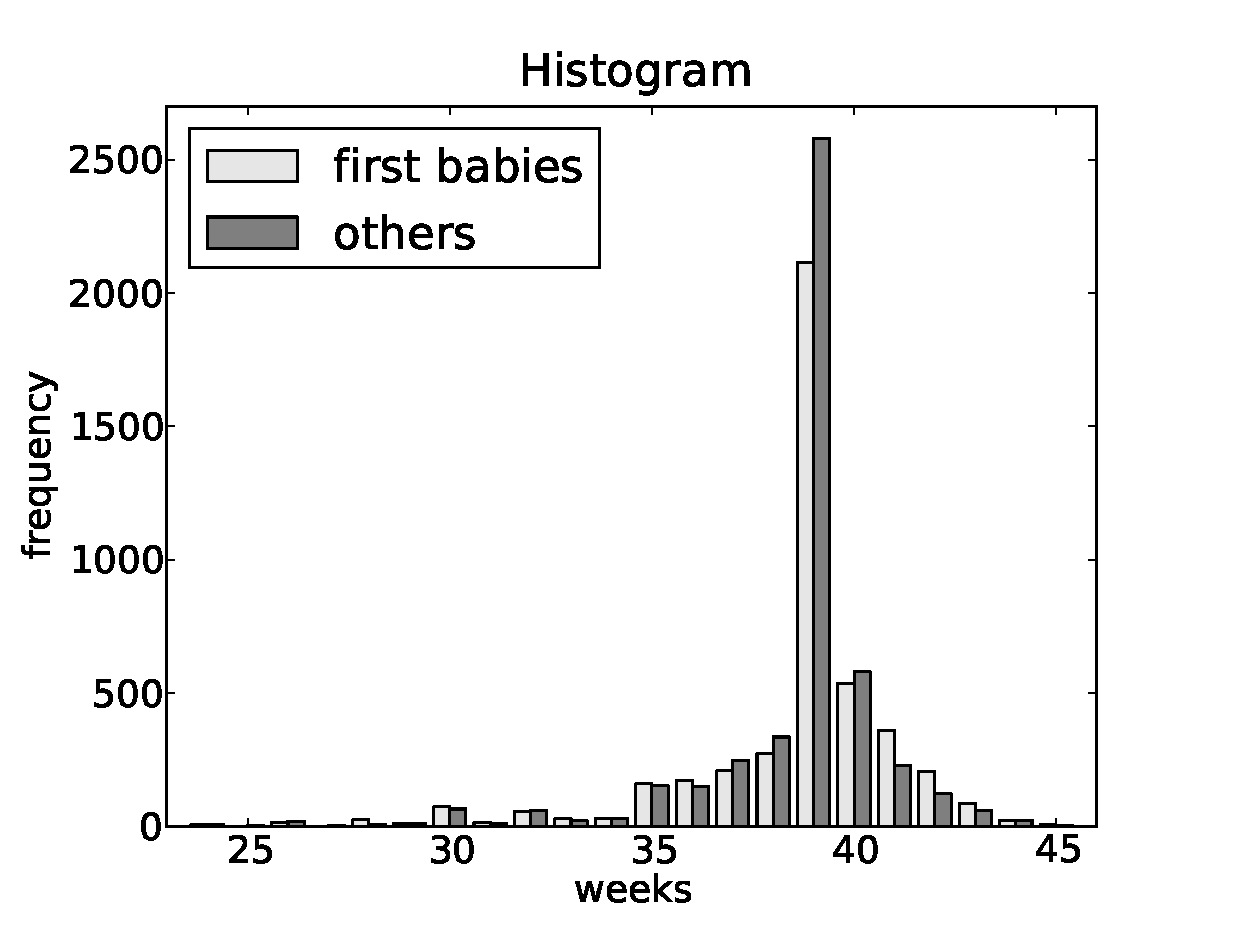
\includegraphics[height=2.5in]{workspace/nsfg_hist.eps}}
\caption{Histogram of pregnancy lengths.}
\label{nsfg_hist}
\end{figure}

Histograms are useful because they make the following features immediately
apparent:

\begin{description}

\item[Mode:]  The most obvious feature of this distribution is the large
number of values at 39 weeks.  The most common value in a distribution is
called the {\bf mode}.  In this case, the mode is the summary statistic
that does the best job of describing the typical value.

\item[Shape:] Around the mode, the distribution is asymmetric; it drops
off quickly to the right and more slowly to the left.  From a medical
point of view, this makes sense.  Babies are often born early, but
seldom later than 42 weeks.  Also, the right side of the distribution is
probably truncated because doctors often intervene after 42 weeks.

\item[Outliers:] Values far from the mode are called {\bf outliers}.
Some of these are just unusual cases, like babies born at 30 weeks.
But many of them are probably due to errors, either in the reporting
or recording of data.

\end{description}

Although histograms make some features apparent, they are usually not
useful for comparing two distributions.  In this example, there are
fewer ``first babies'' than ``others,'' so some of the apparent
differences in the histograms are due to sample sizes.


\section{Plotting PMFs}

We can solve that problem by normalizing the distributions---that
is, dividing through by the sample sizes---to generate the PMFs.
Figure~\ref{nsfg_pmf} shows the result.

\begin{figure}
% descriptive.py
\centerline{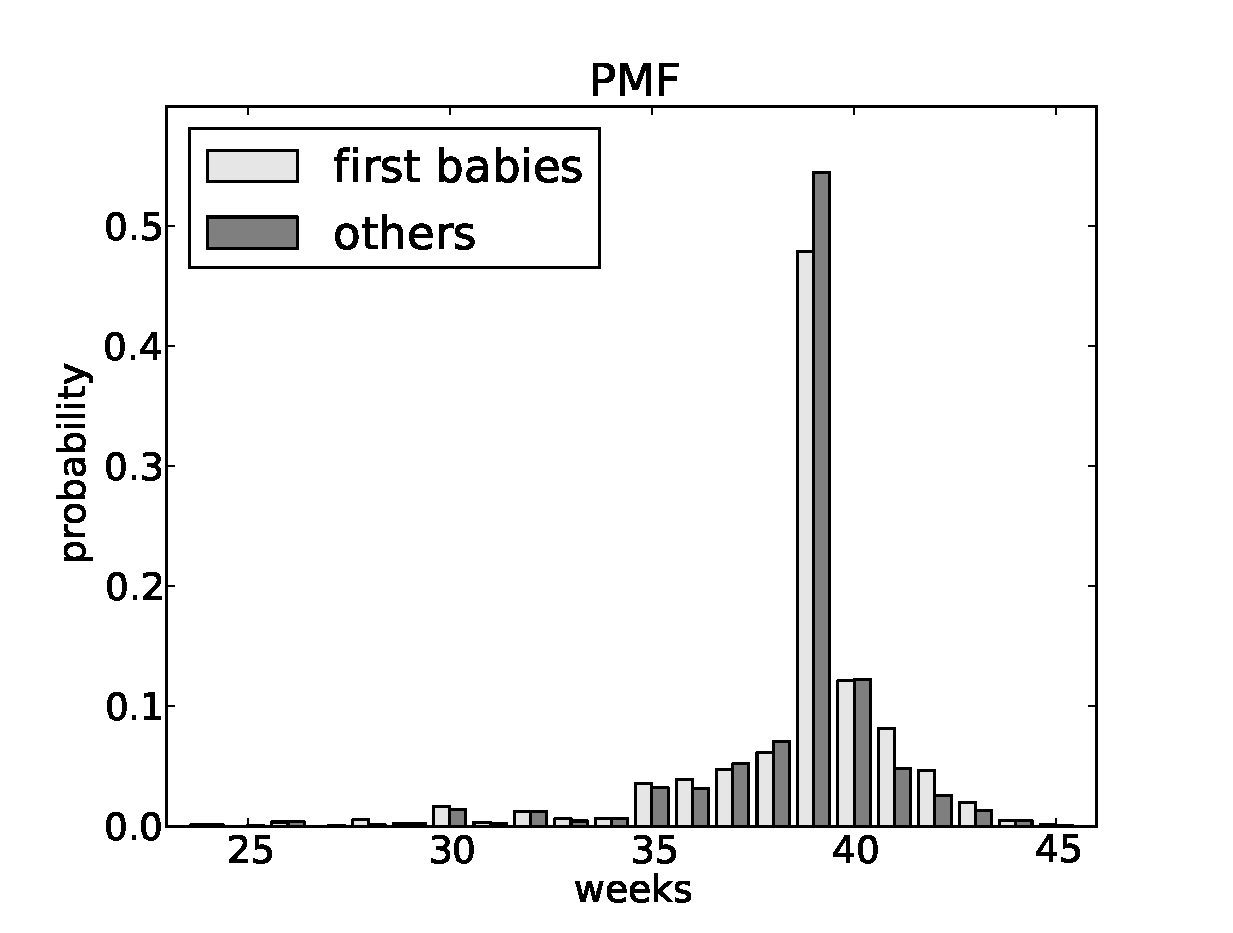
\includegraphics[height=2.5in]{workspace/nsfg_pmf.eps}}
\caption{PMF of pregnancy lengths.}
\label{nsfg_pmf}
\end{figure}

Using the PMF, we can see more clearly where the distributions
differ.  First babies seem to be less likely to arrive on time
(week 39) and more likely to be a little late (weeks 41 and 42).

\begin{ex}
Create a file named {\tt plot.py} and write a function called {\tt
  Hist} that takes a Hist object and generates a bar chart using {\tt
  pyplot.bar}.  This function should also work for Pmf objects.

Write another function called {\tt Hists} that takes two Hists (or Pmfs)
and generates side-by-side histograms like the figures in this
section.  You will have to read the {\tt pyplot} documentation to
adjust the width and position of the bars.

Use the data from the NSFG to generate plots like the ones in this
section.
\end{ex}


\section{Outliers}

Outliers are values that are far from the mode.  Outliers might
be caused by errors in collecting or processing the data, or
they might be legitimate, if unusual, measurements.

It is always a good idea to check for outliers, and sometimes
it is useful, and appropriate, to discard them.

In the list of pregnancy lengths for live births, the 10 lowest values are

\begin{verbatim}
weeks  count
0      1
4      1
9      1
13     1
17     2
18     1
19     1
20     1
21     2
22     7
\end{verbatim}

Values below 20 weeks are certainly errors, and values higher than 30
weeks are probably legitimate.  But there are a non-negligible number of
values in between that are hard to interpret.

On the other end, the 10 highest values are

\begin{verbatim}
weeks  count
40     1116
41     587
42     328
43     148
44     46
45     10
46     1
47     1
48     7
50     2
\end{verbatim}

Again, there are some values here that are almost certainly errors, but
it is hard to know for sure.

Correcting other errors (like the bump at 35 weeks)?
   (use birth weight?)

Trimmed mean and variance.

Don't get carried away.


\section{Other visualizations}

Histograms and PMFs are useful for exploratory data analysis;
once you have an idea what is going on, it is often useful to
design a visualization that focuses on the apparent effect.

In the NSFG data, the biggest differences in the distributions are
near the mode.  So it makes sense to zoom in on that part of the
graph, and to transform the data to emphasize differences.

Figure~\ref{nsfg_diffs} shows the difference between the PMFs for weeks
35-45.  I multiplied by 100 to express the differences in percentage
points.

\begin{figure}
% ???
\centerline{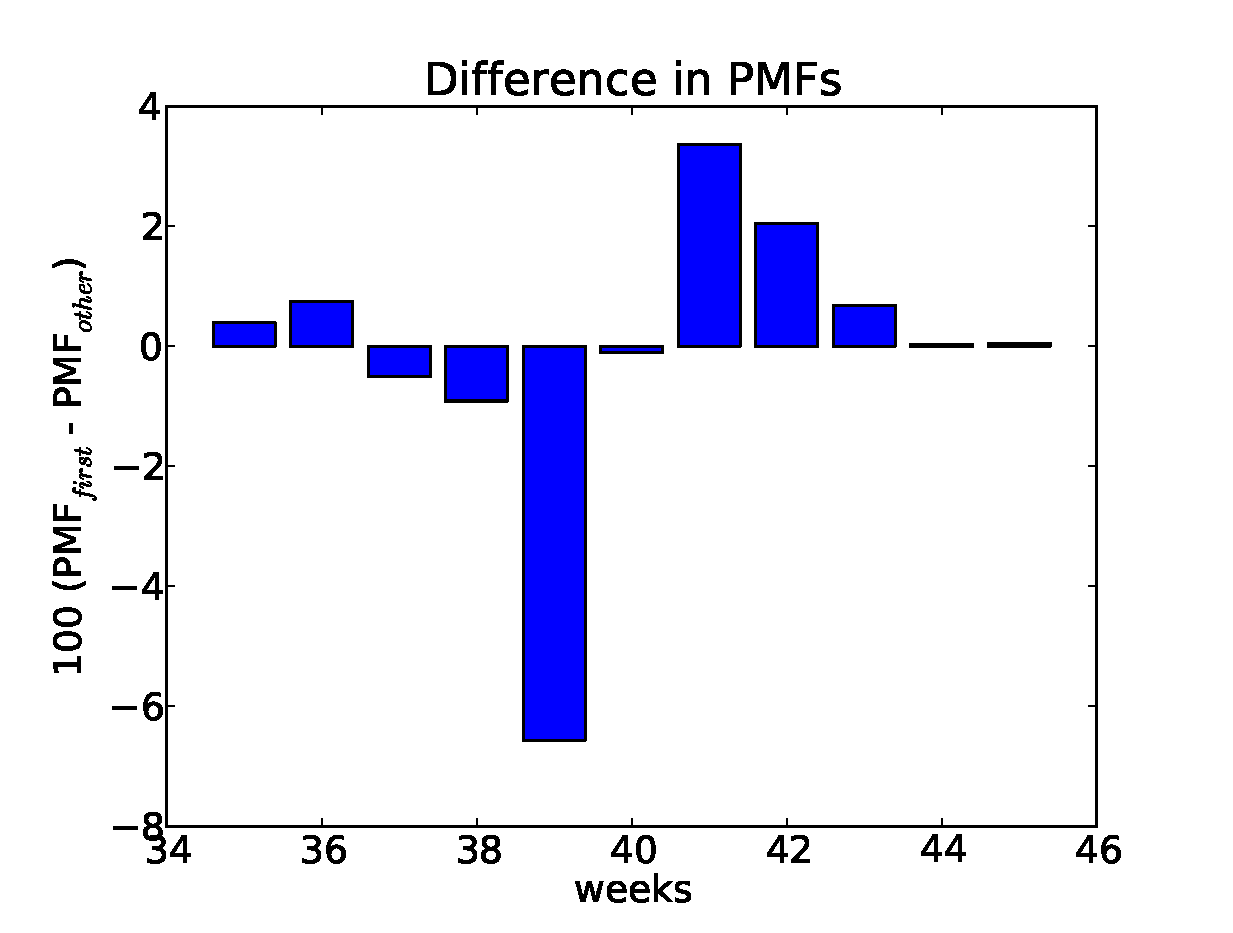
\includegraphics[height=2.5in]{workspace/nsfg_diffs.eps}}
\caption{Difference in percentage, by week.}
\label{nsfg_diffs}
\end{figure}

This figure makes the pattern clearer: first babies are
less likely to be born in week 39, and somewhat more likely
to be born in weeks 41 and 42.


\section{Relative risk}

We started with the question, ``Do first babies arrive late?''  To
make that more precise, let's say that a baby is early if it is born
during Week 37 or earlier, on time if it is born during Week 38, 39 or
40, and late if it is born during Week 41 or later.  Ranges like these
that are used to group data are called {\bf buckets}.

\begin{ex}

Create a file named {\tt risk.py}.
Write functions named {\tt ProbEarly}, {\tt ProbOnTime} and
{\tt ProbLate} that take a PMF and compute the fraction of births
that fall into each bucket.  Hint: write a generalized function
that these functions call.

Make three PMFs, one for first babies, one for others, and one for
all live births.  For each PMF, compute the probability of being
born early, on time, or late.

One way to summarize data like this is with a {\bf relative risk},
which is a ratio of two probabilities.  For example, the probability
that a first baby is born early is 18.2\%.  For other babies it is
16.8\%, so the relative risk is 1.08.  That means that first babies
are about 8\% more likely to be early.

Write code to confirm those results, then compute the relative risks of
being born on time and being late.

\end{ex}


\section{Conditional probability}

Imagine that someone you know is pregnant, and it is the beginning of
Week 39.  What is the chance that the baby will be born in the next
week?  How much does the answer change if it's a first baby?

We can answer these questions by computing a {\bf conditional
probability}, which is (ahem!) a probability that depends on a condition.
In this case, the condition is that we know the baby didn't arrive
during Weeks 0--38.

Here's one way to do it:

\begin{enumerate}

\item Given a PMF, generate a fake cohort of 1000 pregnancies.
For each number of weeks, $x$, the number of pregnancies with
duration $x$ is $1000 PMF(x)$.

\item Remove from the cohort all pregnancies with length less than 39.

\item Compute the PMF of the remaining durations; the result is the
conditional PMF.

\item Evaluate the conditional PMF at $x = 39$ weeks.

\end{enumerate}

\begin{ex}
Create a file named {\tt conditional.py}.
Write a program that implements this algorithm and computes the
probability that a baby will be born during Week 39, given that
it was not born prior to Week 39.

Generalize this program to compute the
probability that a baby will be born during Week $x$, given that
it was not born prior to Week $x$, for all $x$.

Plot this value as a function of $x$ for first babies and others.

\end{ex}


\section{Reporting results}

At this point we have explored the data and seen several apparent
effects.  For now, let's assume that these effects are real (but let's
remember that it is an assumption).  How should we report these
results?

The answer might depend on who is asking the question.  For example,
a scientist might be interested in any (real) effect, no matter how
small.  A doctor might only care about effects that are
{\bf clinically significant}; that is, differences that make a difference.
A pregnant woman might be interested in results that are relevant to
her, like the conditional probabilities in the previous section.

How you report results might also depend on your goals.  If you are
trying to demonstrate the significance of an effect, you might choose
summary statistics, like relative risk, that emphasize differences.
If you are trying to reassure a patient, you might choose statistics
that put the differences in context.

\begin{ex}

Based on the results from the previous exercises, suppose you were
asked to summarize what you learned about whether first
babies arrive late.

Which summary statistics would you use if you wanted to get a story
on the evening news?  Which ones would you use if you wanted to
reassure an anxious patient?

Finally, imagine that you are Cecil Adams, author of {\it The Straight
  Dope} (\url{straightdope.com}), and your job is to answer the
question, ``Do first babies arrive late?''  Write a paragraph that
uses your results to answer this question clearly, precisely, and
accurately.

\end{ex}


\section{Mean and variance of PMFs}

In Section~\ref{mean} we computed the mean of a sample by adding up
the elements and dividing by $n$.  If you are given a PMF, you can
still compute the mean, but the process is slightly different:

\[ \mu = \sum_i p_i x_i \]

where the $x_i$ are the unique values in the PMF and $p_i = PMF(x_i)$.
Similarly, you can compute variance like this:

\[ \sigma^2 = \sum_i p_i (x_i - mu)^2\]

\begin{ex}
In {\tt Pmf.py}, add methods named {\tt Mean} and {\tt Var} that compute
the mean and variance of a Pmf.

To test these methods, check that they are consistent with the
functions {\tt Mean} and {\tt Var} you wrote in {\tt thinkstats.py}.
\end{ex}


\section{The class size paradox}

At many American colleges and universities, the student-to-faculty
ratio is about 10:1.  But students are often surprised to discover
that their average class size is (much) bigger than 10.  There
are two reasons for the discrepancy:

\begin{itemize}

\item Students typically take 4--5 classes per semester, but
professors often teach 1 or 2.

\item The number of students who enjoy a small class is small,
but the number who suffer in a large class is large.

\end{itemize}

The first effect is obvious (at least once it is pointed out);
the second is more subtle.  So let's look at an example.  Suppose
that a college offers 65 classes in a given semester, with the
following distribution of sizes:

\begin{verbatim}
Sizes        Count
-----        -----
 0- 4          0
 5- 9          8
10-14          8
15-19         14
20-24          4
25-29          6
30-34         12
35-39          8
40-44          3
45-49          2
\end{verbatim}

If you ask the Dean for the average class size, he would
construct a PMF, compute the mean, and report that the
average class size is 24.

But if you survey a group of students, ask them how many
students are in their classes, and compute the mean, you would
conclude that the average class size is 29.

\begin{ex}
Build a PMF of these data and compute the mean.  Now compute the
average class size as perceived by students.

Note: since the data have been rounded off, you can use the mid-point
of each range.  
\end{ex}


\section{Glossary}


\chapter{Cumulative distribution functions}

\section{The limits of PMFs}

In general PMFs work well if the number of different values is less than
about 50.  But as the number of possible values increases, the probability
associated with each value gets smaller and the effect of random noise
increases.

For example, we might be interested in the distribution of birth
weights.  In the NSFG, the integer variables \verb"birthwgt_lb" and
\verb"birthwgt_oz" encode birth weight in pounds and ounces.
Figure~\ref{nsfg_birthwgt_pmf} shows the PMF of these values,
converted to total weight in ounces, for first babies and others.

\begin{figure}
% cumulative.py
\centerline{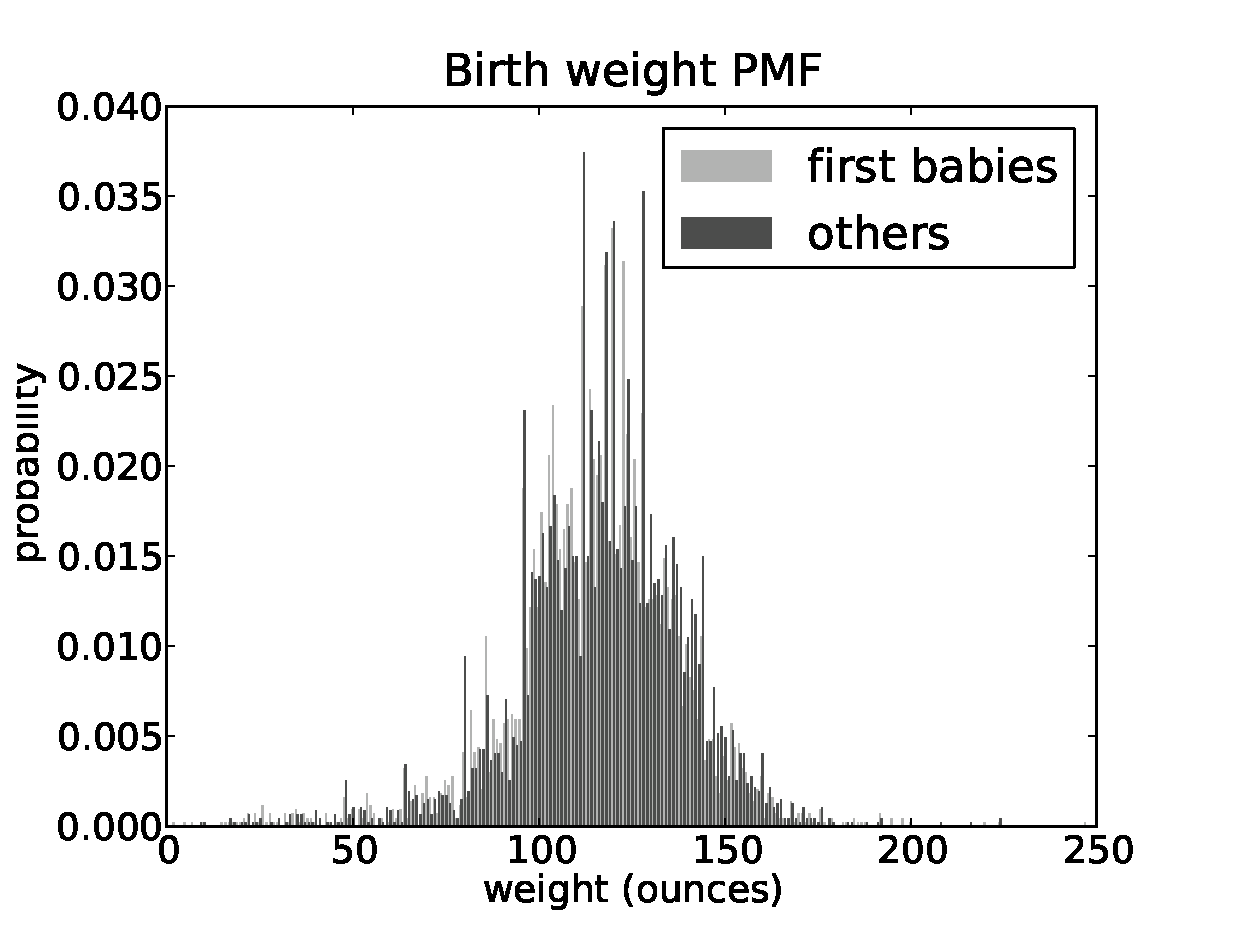
\includegraphics[height=2.5in]{workspace/nsfg_birthwgt_pmf.eps}}
\caption{PMF of birth weights.}
\label{nsfg_birthwgt_pmf}
\end{figure}

Overall, these distributions resemble the familiar ``bell curve,'' with
many values near the mean and a few values much higher and lower.

But parts of this figure are hard to interpret.  There are many spikes
and valleys, and some apparent differences between the distributions.
But it hard to tell which of these features are significant.  Also, it
is hard to see overall patterns; for example, which distribution do
you think has the higher mean?

These problems can be mitigated by {\bf binning} the data;
that is, dividing the domain into non-overlapping intervals and counting
the number of values in each ``bin.''  Binning can be useful, but it is
tricky to get the size of the bins right.  If they are big enough to
smooth out noise, they might also smooth out useful information.

An alternative that avoids these problems is the {\bf cumulative
distribution function}, or {\bf CDF}.  But before we can get to that,
we have to talk about percentiles.


\section{Percentiles}

If you have taken a standardized test, you probably got your
results in the form of a raw score and a {\bf percentile rank}.
In this context, the percentile rank is the fraction of people who
scored lower than you (or the same).  So if you are ``in the 90th
percentile,'' you did as well as or better than 90\% of the people who
took the exam.

Here's how you could compute the percentile rank of a value,
\verb"your_score", relative to the scores in the sequence {\tt
  scores}:

\begin{verbatim}
def PercentileRank(scores, your_score):
    count = 0
    for score in scores:
        if score <= your_score:
            count += 1

    percentile_rank = 100.0 * count / len(scores)
    return percentile_rank
\end{verbatim}
%
% see score_example.py
%
For example, if the scores in the sequence were 55, 66, 77, 88 and 99,
and you got the 88, then your percentile rank would be {\tt 100 * 4 / 5}
which is 80.

If you are given a value, it is easy to find its percentile rank; going
the other way is slightly harder.  If you are given a percentile rank
and you want to find the corresponding value, one option is to
sort the values and search for the one you want:

\begin{verbatim}
def Percentile(scores, percentile_rank):
    scores.sort()
    for score in scores:
        if PercentileRank(scores, score) >= percentile_rank:
            return score
\end{verbatim}

The result of this calculation is a {\bf percentile}.  For example,
the 50th percentile is the value with percentile rank 50.  In the
distribution of exam scores, the 50th percentile is 77.

\begin{ex}
This implementation of {\tt Percentile} is not very efficient.  A
better approach is to use the percentile rank to compute the index of
the corresponding percentile.  Write a version of {\tt Percentile} that
uses this algorithm.
\end{ex}

\begin{ex}
This exercise is optional.

If you only want to compute one percentile, it is not efficient
to sort the scores.  A better option is the selection algorithm,
which you can read about at \url{wikipedia.org/wiki/Selection_algorithm}.

Write (or find) an implementation of the selection algorithm and use
it to write an efficient version of {\tt Percentile}.
\end{ex}


\section{Cumulative distribution functions}

Now that we understand percentiles, we are ready to tackle the
cumulative distribution function (CDF).  The CDF is the function that
maps values to their percentile rank in a distribution.

The CDF is a function of $x$, where $x$ is any value that might appear
in the distribution.  To evaluate $CDF(x)$ for a particular value of
$x$, we compute the fraction of the values in the sample less than (or
equal to) $x$.

Here's what that looks like as a Python function that takes a sample,
{\tt t}, and a value, {\tt x}:

\begin{verbatim}
def Cdf(t, x):
    count = 0.0
    for value in t:
        if value <= x:
            count += 1.0

    prob = count / len(t)
    return prob
\end{verbatim}

This function should look familiar; it is almost identical to {\tt
  PercentileRank}, except that the result is in a probability in the
range 0--1 rather than a percentile rank in the range 0--100.

As an example, suppose a sample has the values $\{1, 2, 2, 3, 5\}$.
Here are some values from its CDF:

\begin{eqnarray*}
CDF(0) &=& 0    \\
CDF(1) &=& 0.2    \\
CDF(2) &=& 0.6    \\
CDF(3) &=& 0.8    \\
CDF(4) &=& 0.8    \\
CDF(5) &=& 1    \\
\end{eqnarray*}
%
We can evaluate the CDF for any value of $x$, not just
values that appear in the sample.
If $x$ is less than the smallest value in the sample, $CDF(x)$ is 0.
If $x$ is greater than the largest value, $CDF(x)$ is 1.

Figure~\ref{example_cdf} is a graphical representation of this CDF.

\begin{figure}
% Cdf_test.py
\centerline{\includegraphics[height=2.5in]{workspace/example_cdf.eps}}
\caption{Example of a CDF.}
\label{example_cdf}
\end{figure}

The CDF of a sample is a step function.  In the next chapter we
will see distributions whose CDFs are continuous functions.  

The function {\tt Cdf}, above, is efficient enough if we only want
to evaluate the CDF at one point.  But there are several operations
we might want to perform on CDFs:

\begin{description}

\item[Evaluate:] Given a value $x$, evaluate $CDF(x)$ to get a
  probability $p$.  This operation computes percentile ranks.

\item[Invert:] Given a probability $p$, find the value $x$ so that
  $CDF(x) = p$.  This operation computes percentiles.

\item[Render:] Generate a sequence of points suitable for plotting the
  CDF.

\end{description}

It is not obvious what data structures we should use to implement
these operations; there are several reasonable choices.  In the
following exercise I recommend an option that is simple and efficient.

\begin{ex}
Create a file named {\tt Cdf.py} and write a definition for a class
named {\tt Cdf} that represents a CDF.  The attributes of a Cdf
object are {\tt xs}, which is a sorted list of the unique values
in the sample, and {\tt ps} which is a list of probabilities that
correspond to the values in {\tt xs}.

Write a simple constructor that takes {\tt xs} and {\tt ps} as
parameters, then write two functions:

\begin{description}

\item[{\tt MakeCdfFromDict}]: Takes a dictionary that maps from
values to frequencies, computes {\tt xs} and {\tt ps}, and returns
a {\tt Cdf} object.

\item[{\tt MakeCdfFromList}]: Takes a sequence of values, makes
a dictionary that maps from values to frequencies, and uses
{\tt MakeCdfFromDict} to make and return a {\tt Cdf} object.

\end{description}

Now write the following methods for {\tt Cdf}:

\begin{description}

\item[{\tt Prob}]: Given a value $x$, compute the probability $p = CDF(x)$.

\item[{\tt Value}]: Given a probability $p$, compute the
corresponding value, $x$; that is, the inverse CDF of $p$.

\item[{\tt Render}]: Return two lists, {\tt xs} and {\tt ps}, suitable
for plotting the CDF.  Notice that the CDF is a step function, so these
lists should have two elements for each unique value in the distribution.

\end{description}

Test your code by computing the CDF of the values $\{1, 2, 2, 3, 5\}$.
Test {\tt Prob} and {\tt Value} using the examples in this section.

Write a function that plots the CDF with the {\tt pyplot} function
{\tt plot}.  Confirm that your plot looks like the figure above.

You can download a solution from \url{thinkstatsbook.com/Cdf.py}.
\end{ex}


\section{Back to the survey data}

Figure~\ref{nsfg_birthwgt_cdf} shows the CDFs of birth weight for
first babies and others in the NSFG dataset.

\begin{figure}
% cumulative.py
\centerline{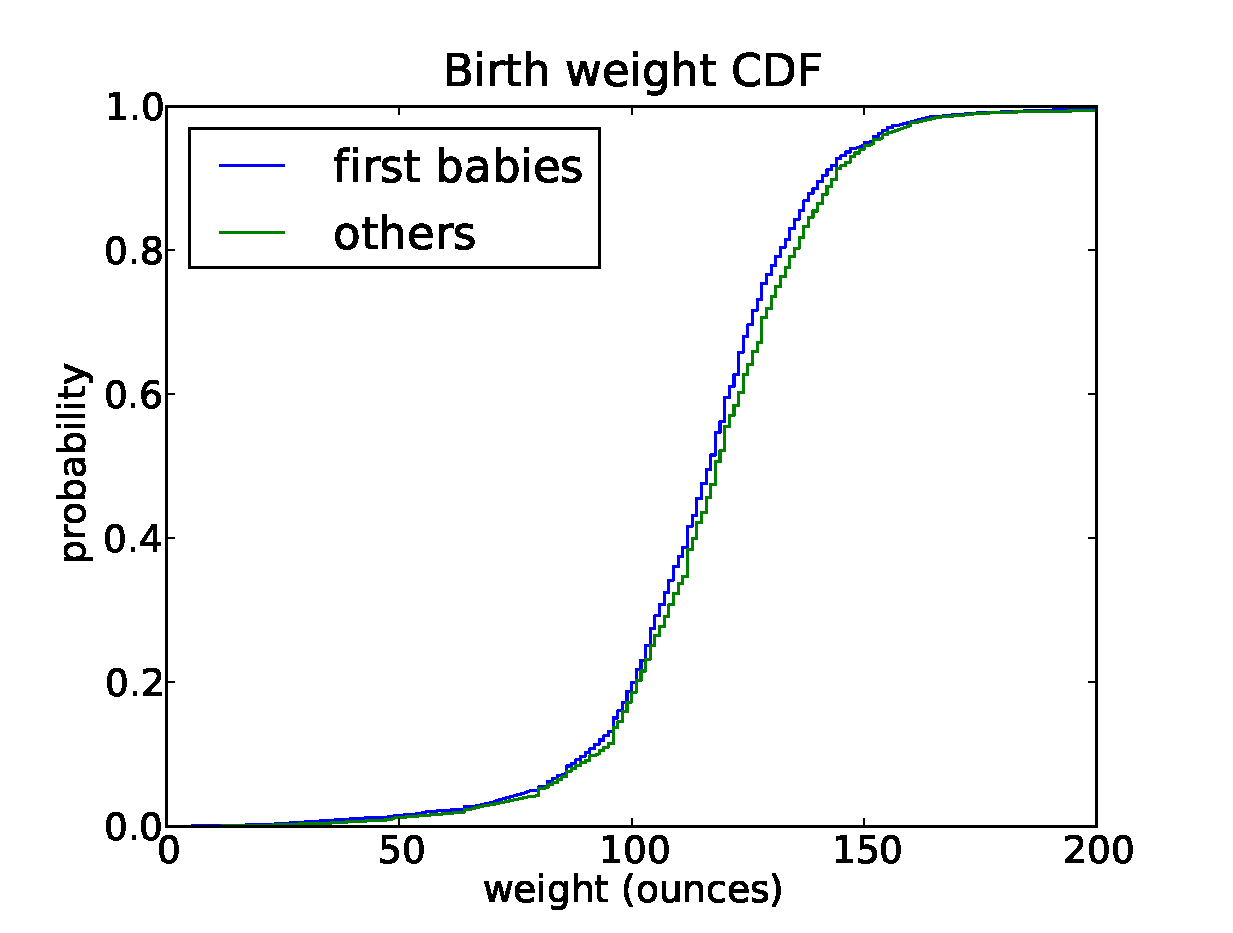
\includegraphics[height=2.5in]{workspace/nsfg_birthwgt_cdf.eps}}
\caption{CDF of birth weights.}
\label{nsfg_birthwgt_cdf}
\end{figure}

This figure makes the shape of the distributions, and the differences
between them, much clearer.  We can see that first babies are slightly
lighter throughout the distribution, with a larger discrepancy above 
the mean.

\begin{ex}
This exercise is optional.  In the figure above, you might notice
a sequence of equally-spaced values with higher frequency than
their neighbors.  See if you can figure out what it going on.
Hint: look at the PMF of \verb"birthwgt_oz".
\end{ex}

\begin{ex}
How much did you weigh at birth?  If you don't know, call your mother
or someone else who knows.  Using the pooled data (all live births),
compute the distribution of birth weights and use it to find your
percentile rank.  If you were a first baby, find your percentile rank
in the distribution for first babies.  Otherwise use the distribution
for others.  How big is the difference between your percentile ranks
in the two distributions?
\end{ex}


\section{Conditional distributions}

A {\bf conditional distribution} is the distribution of a subset of
the data which is selected according to a condition.

For example, if you are above average in weight, but way above average
in height, then you might be relatively light for your height.  Here's
how you could make that claim more precise.

\begin{enumerate}

\item Select a cohort of people who are the same height as you (within
some range).

\item Find the CDF of weight for those people.

\item Find the rank percentile of your weight in that distribution.

\end{enumerate}


\begin{ex}
Find out how tall (long, actually) you were at birth.  If you don't
know, call your mother again.  Find the CDF of birth weight for
people who were the same height, and compute your percentile rank
in that CDF.

Now find the rank percentile of your height conditioned on your weight.
\end{ex}


\section{Age group ranking}

Percentile ranks are useful for comparing measurements from different
tests, or tests applied to different groups.

For example, people who compete in foot races are usually grouped by
age and gender.  To compare people in different groups, you can convert
race times to percentile ranks.

\begin{ex}

I recently ran in the 27th Anniversary Edition James Joyce Ramble 10K
in Dedham MA.  The results are available from
\url{coolrunning.com/results/10/ma/Apr25_27thAn_set1.shtml}.
Go to that page and find my results.  I came in 97th in a field
of 1633, so what is my percentile rank in the field?

In my division (M4049 means ``male between 40 and 49 years of age'')
I came in 26th out of 256.  What is my percentile rank in my division?
What does that tell you about my division?

If I am still running in 10 years (and I hope I am), I will be in
the M5059 division.  Assuming that my percentile rank in my division
is the same, how much slower should I expect to be?

I maintain a friendly rivalry with a student of mine who is in the
F2039 division.  How fast does she have to run her next 10K to
``beat'' me in terms of percentile ranks?

\end{ex}

\section{Random numbers}

CDFs are also useful for generating random numbers
with a given distribution.  Here's how:

\begin{itemize}

\item Choose a random probability in the range 0--1.

\item Use {\tt Cdf.Value} to find the value in the distribution
that corresponds to the probability you chose.

\end{itemize}

It might not be obvious why this works, but since it is easier
to implement than explain, let's try it out.

\begin{ex}

Add a method to the Cdf class, called {\tt sample}, that takes
an integer {\tt n} and returns a list of $n$ values chosen at
random from the distribution.  Hint: use {\tt random.random}.

Using the distribution of birth weights from the NSFG, generate a
random sample with 1000 elements.  Compute the CDF of the sample.
Make a plot that shows the original CDF and the CDF of the random
sample.  For large values of $n$, the distributions should be
the same.

\end{ex}

This process, generating a random sample based on a measured sample,
is called {\bf resampling}.


\section{Summary statistics revisited}

Once you have computed a CDF, it is easy to compute other summary
statistics.  The median is just the 50th percentile\footnote{You might
see other definitions of the median.  In particular,
some sources suggest that if you have an even number of elements in
a sample, the median is the average of the middle two elements.
This is an unnecessary special case, and it has the odd effect of
generating a value that is not in the sample.  As far
as I'm concerned, the median is the 50th percentile.  Period.}.
The 25th and 75th percentiles are often used to check whether
a distribution is symmetric, and their difference, which is called
the {\bf interquartile range} measures the spread.

\begin{ex}
Compute the 25th, 50th, and 75th percentiles of the birth weight
CDF.  Do these values suggest that the distribution is symmetric?

Add a method to {\tt Cdf}, called {\tt Interquartile}, that computes
the interquartile range.
\end{ex}


\section{Glossary}



\chapter{Continuous distributions}

The distributions we have used so far are called {\bf
  empirical distributions} because they are based on empirical
observations.

The alternative is a {\bf continuous distribution}, which is
characterized by a CDF that is a continuous function (as opposed to a
step function).  Many real world phenomena can be approximated by
continuous distributions, which is why they are useful.

\section{The exponential distribution}

We will start with the exponential distribution because it is
easy to work with.  In the real world, exponential distributions
come up when we look at a series of events and measure the
times between events, which are called {\bf interarrival times}.
If the events are equally likely to occur at any time, the distribution
of interarrival times tends to look like an exponential distribution.

The CDF of the exponential distribution is:

\[ CDF(x) = 1 - e^{-\lambda x} \]

The parameter, $\lambda$, determines the shape of the
distribution.  Figure~\ref{expo_cdf} shows what this CDF looks like with
$\lambda = 2$.

\begin{figure}
\centerline{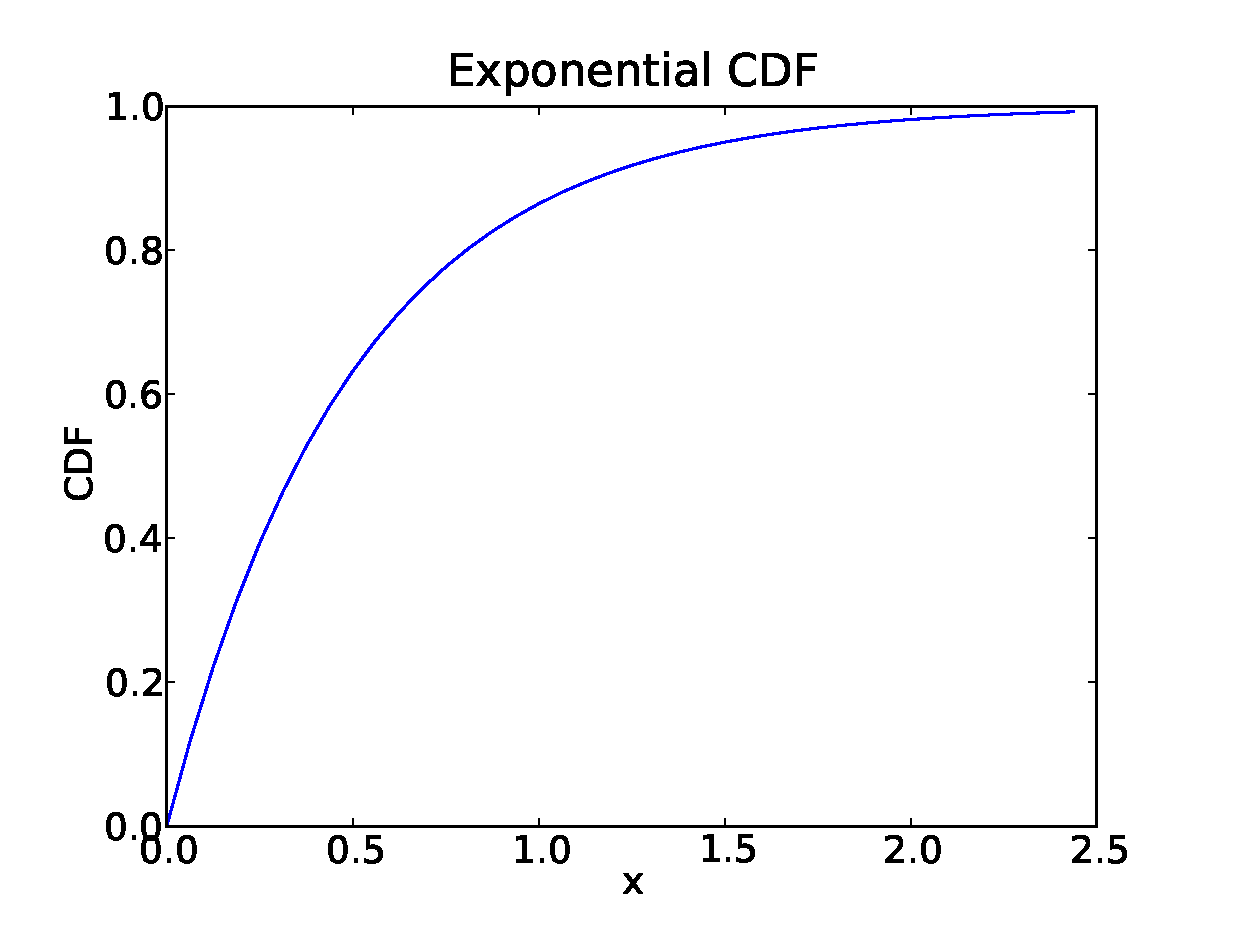
\includegraphics[height=2.5in]{workspace/expo_cdf.eps}}
\caption{CDF of exponential distribution.}
\label{expo_cdf}
\end{figure}

In general, the mean of an exponential distribution is $1 / \lambda$,
so the mean of this distribution is 0.5.  The median is $log(2) / \lambda$,
which is roughly 0.35.

To see an example of a distribution that is approximately exponential,
we will look at the interarrival time of babies.
On December 18, 1997, 44 babies were born in a hospital in Brisbane,
Australia\footnote{This example is based on information and data from
  Dunn, ``A Simple Dataset for Demonstrating Common Distributions,''
  Journal of Statistics Education v.7, n.3 (1999).}.  The times of
birth for all 44 babies were reported in the local paper; you can
download the data from \url{thinkstatsbook.com/babyboom.dat}.

Figure~\ref{interarrivals} shows the CDF of the interarrival times
in minutes.  It seems to have the general shape of an exponential
distribution, but how can we tell?

\begin{figure}
\centerline{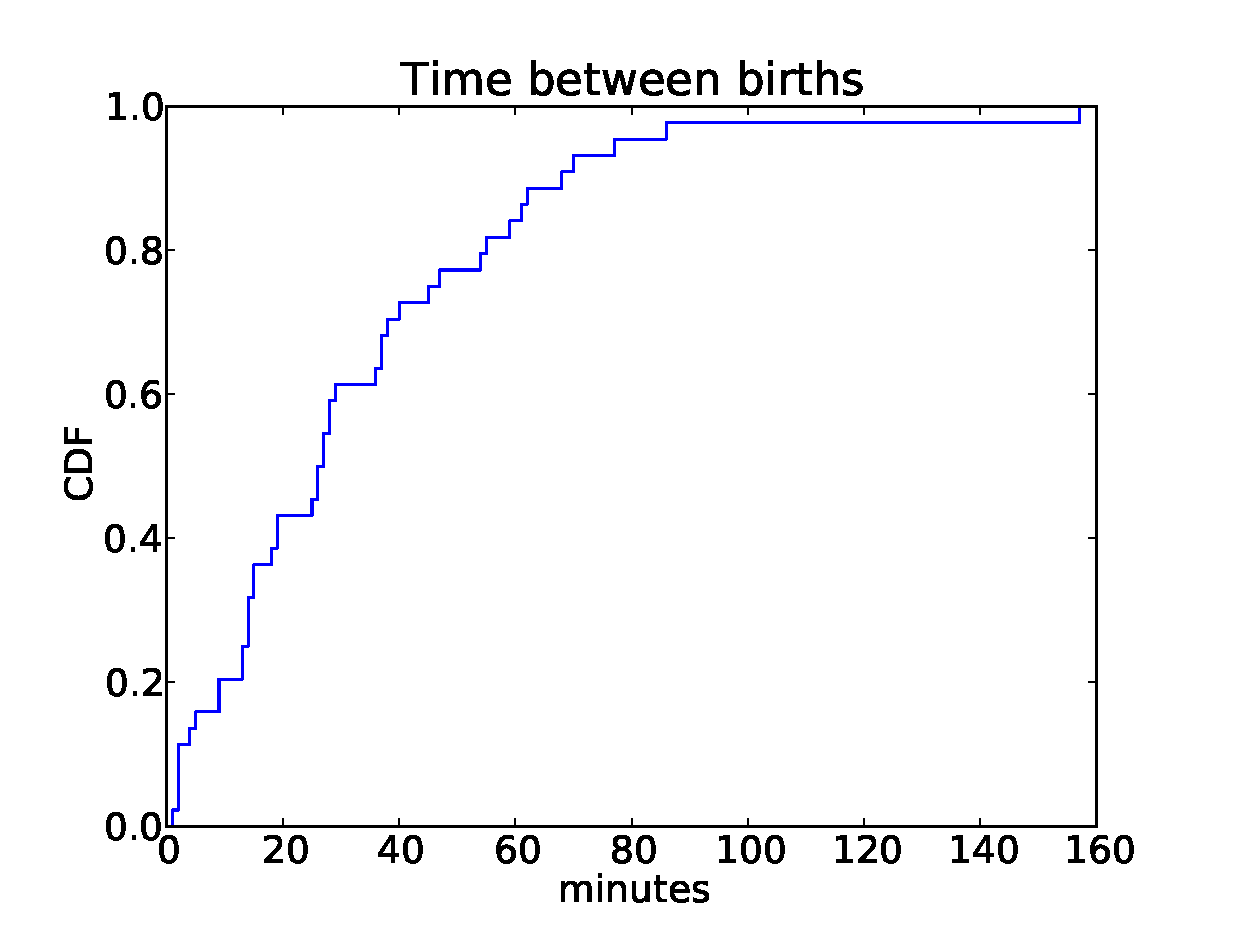
\includegraphics[height=2.5in]{workspace/interarrivals.eps}}
\caption{Interarrival times.}
\label{interarrivals}
\end{figure}

One way is to plot the complementary CDF, which is $1 - CDF(x)$, on a
log-$y$ scale.  For data from an exponential distribution, the result
is a straight line.  Let's see why that works...

If you plot the complementary CDF of a dataset that you think is
exponential, you expect to see a function like:

\[ y = \sim e^{-\lambda x} \]

If you take the log of both sides of this equation, you get:

\[ \log y \sim -\lambda x \]

So on a log-$y$ scale the complementary CDF is a straight line
with slope $-\lambda$.

Figure~\ref{interarrivals_logy}
shows the complementary CDF on a
log-$y$ scale.  It is not exactly straight, which suggests that
the exponential model is only an approximation of the observed
process.  Most likely the underlying assumption---that a birth is
equally likely at any time of day---is not exactly true.

\begin{figure}
\centerline{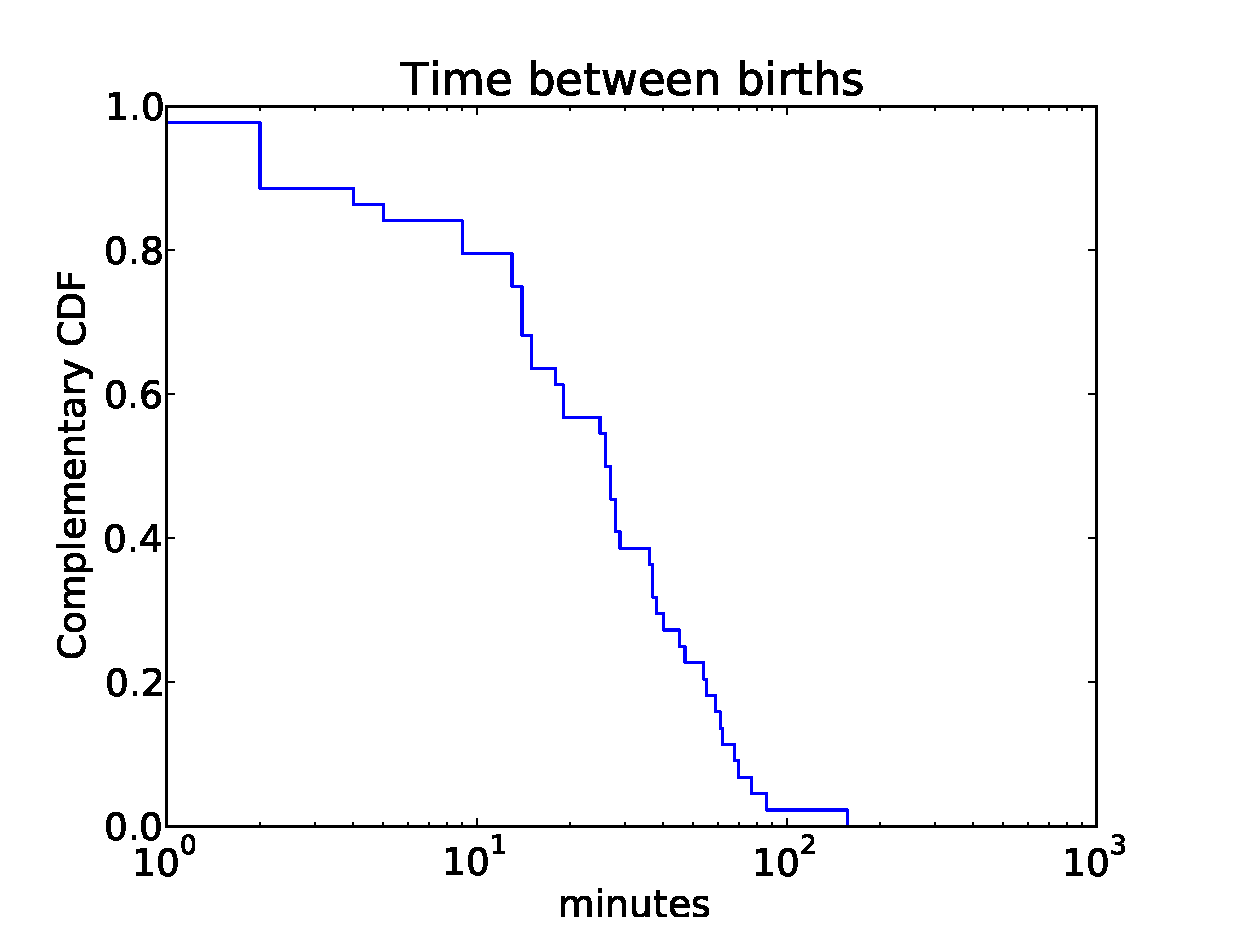
\includegraphics[height=2.5in]{workspace/interarrivals_logy.eps}}
\caption{Interarrival times.}
\label{interarrivals_logy}
\end{figure}

\begin{ex}
For small values of $n$, we don't expect an empirical distribution
to fit a continuous distribution exactly.  So one way to evaluate
the quality of fit is to generate a sample from a continuous
distribution and see how well it matches the data.

The function {\tt expovariate} in the {\tt random} module
generates random values from an exponential distribution with
a given value of $\lambda$.

Use it to generate 44 values from an exponential distribution with
mean 32.6.  Plot the complementary CDF on a log-$y$ scale and compare
it to Figure~\ref{interarrivals_logy}.

Hint: use the function {\tt pyplot.yscale} to set the scale of the
$y$ axis.
\end{ex}

\begin{ex}
Most people don't know what time they were born, but most people know
their birthday.

Collect the birthdays of the students in your class, sort them, and
compute the interarrival times.  Plot the CDF of the interarrival
times and the complementary CDF on a log-$y$ scale.  Does it look like
an exponential distribution?
\end{ex}


\section{The Pareto distribution}

The Pareto distribution is named after the economist Vilfredo
Pareto, who used it to describe the distribution of wealth
(see \url{wikipedia.org/wiki/Pareto_distribution}).  Since then,
people have used it to describe
a variety of phenomena in the natural and social sciences,
including sizes of cities and towns, sand particles
and meteorites, forest fires and earthquakes.

The Pareto distribution is characterized by a CDF with the following
functional form:

\[ CDF(x) = 1- \left( \frac{x}{x_m} \right) ^{-\alpha} \]

The parameters $x_m$ and $\alpha$ determine the location and shape of
the distribution.  $x_m$ is the minimum possibile quantity.

Values from a Pareto distribution often have these properties:

\begin{description}

\item[Long tail:] Pareto distributions contain many small values
and a few very large ones.  

\item[80/20 rule:] The large values in a Pareto distribution are
so large that they add up to a disproportionate share of the total.
In the context of wealth, the 80/20 rule says that 20\% of the
people own 80\% of the wealth.

\item[Scale free:] If a distribution has a central tendency,
the typical value is also called a {\bf scale}.  For example, the
great majority of adult humans are between 100 and 200 cm in height,
so we could say that the scale of human height is a few hundred
centimeters.  But for long-tailed distributions, there is no
similar range (bounded by a factor of two) that contains the
bulk of the distribution.  So we say that these distributions
are {\bf scale-free}.

\end{description}

To get a sense of the difference between the Pareto and Gaussian
distributions, imagine what the world would be like if the
distribution of human height were Pareto.  Using the same minimum
height, $x_m = 100$ cm, we could choose $\alpha = 1.7$, so that the median
height is about 150 cm.

Here are empirical CDFs for samples with $n=9000$ drawn 
from these two distributions:

XXX HEIGHT CDF.eps

%\begin{figure}
%\centerline{\includegraphics[width=5.5in]{workspace/height_cdf.eps}}
%\caption{CDFs with the same mean and different tail behavior.}
%\label{height_cdf}
%\end{figure}

The figure on the left is on a log-$x$ scale.  It shows that the
median and lower bounds of the distributions are the same, but
the Pareto distribution has a longer tail.  The figure on the
right is on a log-log scale.  The Pareto distribution is a straight
line except in the extreme tail, where it is noisy because of
the limitations of a finite sample.

If you generate 6 billion random values from the Gaussian distribution
shown in the figure, you would guess that the tallest person in the
world is about 255 cm.  In fact, the tallest currently living person,
Leonid Stadnyk, is 259 cm.

But if you generate 6 billion random values from the Pareto
distribution, you will see that the tallest person in the world could
easily be taller than 80.5 km, which would technically make him or her
an astronaut, at least in the United States (see
\url{wikipedia.org/wiki/Earth's_atmosphere}).  That's what it means to
be scale-free!

There is a simple visual test that can indicate whether an empirical
distribution is well-characterized by a Pareto distribution: on a
log-log scale, the CCDF looks like a straight line.  The derivation is
similar to what we saw in the previous section.

The equation for the CCDF is:

\[ y = 1 - cdf(x) \sim \left( \frac{x}{x_m} \right) ^{-\alpha} \]

Taking the log of both sides yields:

\[ \log y \sim -\alpha (\log x - \log x_m ) \]

So if you plot $\log y$ versus $\log x$, it should look like a
straight line with slope $-\alpha$ and intercept $-\alpha \log x_m$.


\begin{ex}
The distribution of populations for cities and towns has been proposed
as an example of a real-world phenomenon that can be described
with a Pareto distribution.

The U.S. Census Bureau publishes data on the population of every
incorporated city and town in the United States.  I have written a
small program that downloads this data and converts it into a
convenient form.  You can download it from
\url{thinkstatsbook.com/populations.py}.  

\begin{enumerate}

\item Read over the program to make sure you know what it does and then
  write a program that computes and plots the distribution of
  populations for the 14593 cities and towns in the dataset.

\item In your {\tt Dist} class, write a function called {\tt quantile}
  that takes a percentile as a parameter and returns the corresponding
  quantity.  What is the median size in this distribution (the
  quantity that corresponds to the 50th percentile)?  What are the
  25th and 75th percentiles?

\item Plot the CDF on linear and log-$x$ scales so you can get a sense
  of the shape of the distribution.  Then plot the CCDF on a log-log
  scale to see if it has the characteristic shape of a Pareto
  distribution.

\item Use your plot to estimate values for the parameters $x_m$ and
  $\alpha$.  Then use the function {\tt paretovariate} in the {\tt random}
  module to generate 14593 values from a Pareto distribution with the
  parameters you estimated in the previous problem.  Plot the CCDF on
  a log-log scale and compare it the CCDF of the observed data.

\end{enumerate}

What conclusion do you draw about the distribution of sizes
for cities and towns?

\end{ex}

\begin{ex}

The Weibull distribution is a generalization of the exponential
distribution that comes up in failure analysis
(see \url{wikipedia.org/wiki/Weibull_distribution}).

Can you find a transformation that makes a Weibull distribution look
like a straight line?  What do the slope and intercept of the
line indicate?

Use {\tt random.weibullvariate} to generate a sample from a
Weibull distribution and use it to test your transformation.

\end{ex}




\section{The Normal Distribution}

Most common

Not closed form, but good enough

The birth weight CDF has the characteristic sigma-shaped curve of the
{\bf normal distribution}, also known as the Gaussian distribution.
Strictly speaking, the normal distribution is {\bf continuous}, which means
it is defined for all real values; the birth weight data is discrete,
because it only contains integer values.  But the normal distribution
is often a good approximation of discrete data.


\chapter{Hypothesis testing}

When something unusual happens, people often say something
like, ``Wow!  What were the chances of {\em that}!''  This question
makes sense because we have an intuitive sense that some things
are more likely than others.  But this intuition doesn't
always hold up to scrutiny.

For example, supposed I toss a coin 10 times, and after each I write
down H for heads and T for tails.  If the result was a sequence like
THHTHTTTHH, you would't be to surprised.  But if the result was
HHHHHHHHHH, you would say something
like, ``Wow!  What were the chances of {\em that}!''

In this case, I could answer your question.  The probability of
getting the sequence HHHHHHHHHH is one
in 1024.  But here's the catch, the probability of getting THHTHTTTHH
is also one in 1024, and likewise for any other sequence.

it comes up
heads every time, you would be surprised.  

moments

modes

   multimodal distributions (artifact examples: heights, gestation)




(Something uniform?)

Birth weights

Interarrival time between babies

(something lognormal?)

Sizes of towns


Gelman's paradox
\url{http://www.iq.harvard.edu/blog/sss/archives/2008/04/gelmans_paradox.shtml}

\printindex

\clearemptydoublepage
%\blankpage
%\blankpage
%\blankpage


\end{document}
